\input{_eval.latex}
%%%%%%%%%%%%%%%%
\def\Classe{1STMG}
\def\Titre{Évaluation : Suites numériques}
\def\NoterSur{20}
%%%%%%%%%%%%%%%%
\begin{document}
\DoTitle
\exo{Chapitre précédent - Proportion / évolution \exosur{4}}{
	On donne ci-dessous un extrait de feuille de calcul donnant le nombre d'accidents corporels liés à la sécurité routière en France métropolitaine, de $2011$ à $2013$.

	\begin{center}
		\def\arraystretch{1.6}
		\begin{tabular}{|r|c|c|c|}\hline
			Année                        & $2011$ & $2012$   & $2013$   \\ \hline
			Nombre d'accidents corporels & ...    & $60~437$ & $56~812$ \\ \hline
		\end{tabular}
	\end{center}
	\vspace*{3mm}
	\begin{enumerate}
		\q{1} Donner le pourcentage d'évolution du nombre d'accidents corporels entre $2012$ et $2013$ arrondi à $1\%$ près dixième près.
	\end{enumerate}
	\vspace*{1mm}
	L'évolution du nombre d'accidents corporels de $2013$ à $2014$ a été de $-9,5\%$.
	\begin{enumerate}[resume]
		\q{1}  Déterminer le nombre d'accidents corporels en $2014$ arrondi à l'unité près.
	\end{enumerate}
	\vspace*{1mm}
	L'évolution du nombre d'accidents corporels de $2011$ à $2012$ a été de $-5\%$.
	\begin{enumerate}[resume]
		\q{1} Déterminer le nombre d'accidents corporels en $2011$ arrondi à l'unité près.
		\q{1} Déterminer le taux global d'évolution entre $2011$ et $2013$ arrondi à $0,1\%$ près.
	\end{enumerate}
}
\newpage~\newpage

\exo{Calcul des termes d'une suite \exosur{4}}{
	\vspace{1mm}
	Soit $(u_n)$ , la suite définie pour $n\geq 0$, tel que : $$u_{(n)}=\dfrac{n^2}{2}-3$$
	\be
	\q{1} La suite $(u_n)$ est-elle définie de manière récurrente ou explicite ? Jusitifier.
	\q{2} Calculer les termes $u_{(0)}$ , $u_{(3)}$ et $u_{(10)}$.
	\q{1} Conjecturer le sens de variations de la suite $(u_n)$.
	\ee
}
\newpage

\exo{Suite et indice \exosur{4}}{
	\img{4cm}{img/tab}
	Un indice annuel est modélisé par la suite $(u_n)$ définie sur $\N$ par :
	$$\begin{cases}
			~u_{(0)}=100 \\
			~u_{(n+1)}=1,05\times u_{(n)}-3
		\end{cases}$$
	On désire représenter les premiers termes de cette suite à l'aide d'un tableur.
	\be
	\q{1} Indiquer la formule à saisir en \textbf{B1} et à recopier vers le bas.
	\q{2} Compléter la feuille de calcul ci-contre avec les valeurs de $u_{(1)}$ à $u_{(7)}$.\bi\item Vous détaillerez les calculs uniquement pour $u_{(1)}$ et $u_{(2)}$.\ei
	\q{1} Représenter cette suite pour $n$ compris entre $0$ et $7$ dans le repère présent en annexe.
	\ee
}
\newpage

\exo{Suite et coût de fabrication\exosur{3}}{
	Une entreprise fabrique des chaises. Le coût de fabrication de la $n$-ième chaise, quand elle en a déjà fabriqué $(n-1)$, est donné par : $$C(n)=0,2n^2-2n+10$$
	\be
	\q{1} Établir la listes des coûts de fabrication pour $n$ allant de $1$ à $4$.
	\q{1} Pour $1<n<4$, les coûts de fabrication sont-ils croissants ou décroissants ? Justifier.
	\q{1} Calculer le coût \textbf{total} de fabrication de $4$ chaises.
	\ee
}
\newpage

\exo{Suites et salaire\exosur{5}}{
	Un demandeur d'emploi se voit proposer deux offres :
	\bi
	\item Propoition A : Un salaire initial de $1~150\euro$ par mois et une augmentation de $+3\%$ par an.
	\bi\item On note $(a_n)$ la suite de ces revenus mensuels avec cette proposition.\ei
	\item Propoition B : Un salaire initial de $1~200\euro$ par mois et une augmentation de $10\euro$ par an.
	\bi\item On note $(b_n)$ la suite de ces revenus mensuels avec cette proposition.\ei
	\ei
	\vspace*{2mm}
	\be
	\q{1} Calculer le terme $a_{(2)}$ et $b_{(2)}$ en détaillant vos calculs (arrondir à l'euro près).
	\q{1} Exprimer $a_{(n+1)}$ en fonction de $a_{(n)}$.
	\q{2} Compléter, sans justification le tableau ci-dessous.
	\ee
	\begin{center}
		\def\arraystretch{1.6}
		\begin{tabular}{|r|c|c|c|c|c|c|c|}\hline
			Année     & $1$     & $2$                  & $3$                  & $4$                  & $5$                  \\ \hline
			Salaire A & $1~150$ & $\qquad\qquad\qquad$ & $\qquad\qquad\qquad$ & $\qquad\qquad\qquad$ & $\qquad\qquad\qquad$ \\ \hline
			Salaire B & $1~200$ & $\qquad\qquad\qquad$ & $\qquad\qquad\qquad$ & $\qquad\qquad\qquad$ & $\qquad\qquad\qquad$ \\ \hline
		\end{tabular}
	\end{center}
	\vspace*{1mm}
	\be
	\q{1} Si le demandeur d'emploi prévoit de rester $6$ ans dans l'entreprise, quelle offre doit-il choisir ? Justifier votre réponse par un calcul.
	\ee

}
\newpage~\newpage\backgroundsetup{contents={}}
~\\~
\begin{center}
	\textbf{\LARGE{Annexe - Exercice n°3}}
\end{center}
~\\~
\begin{center}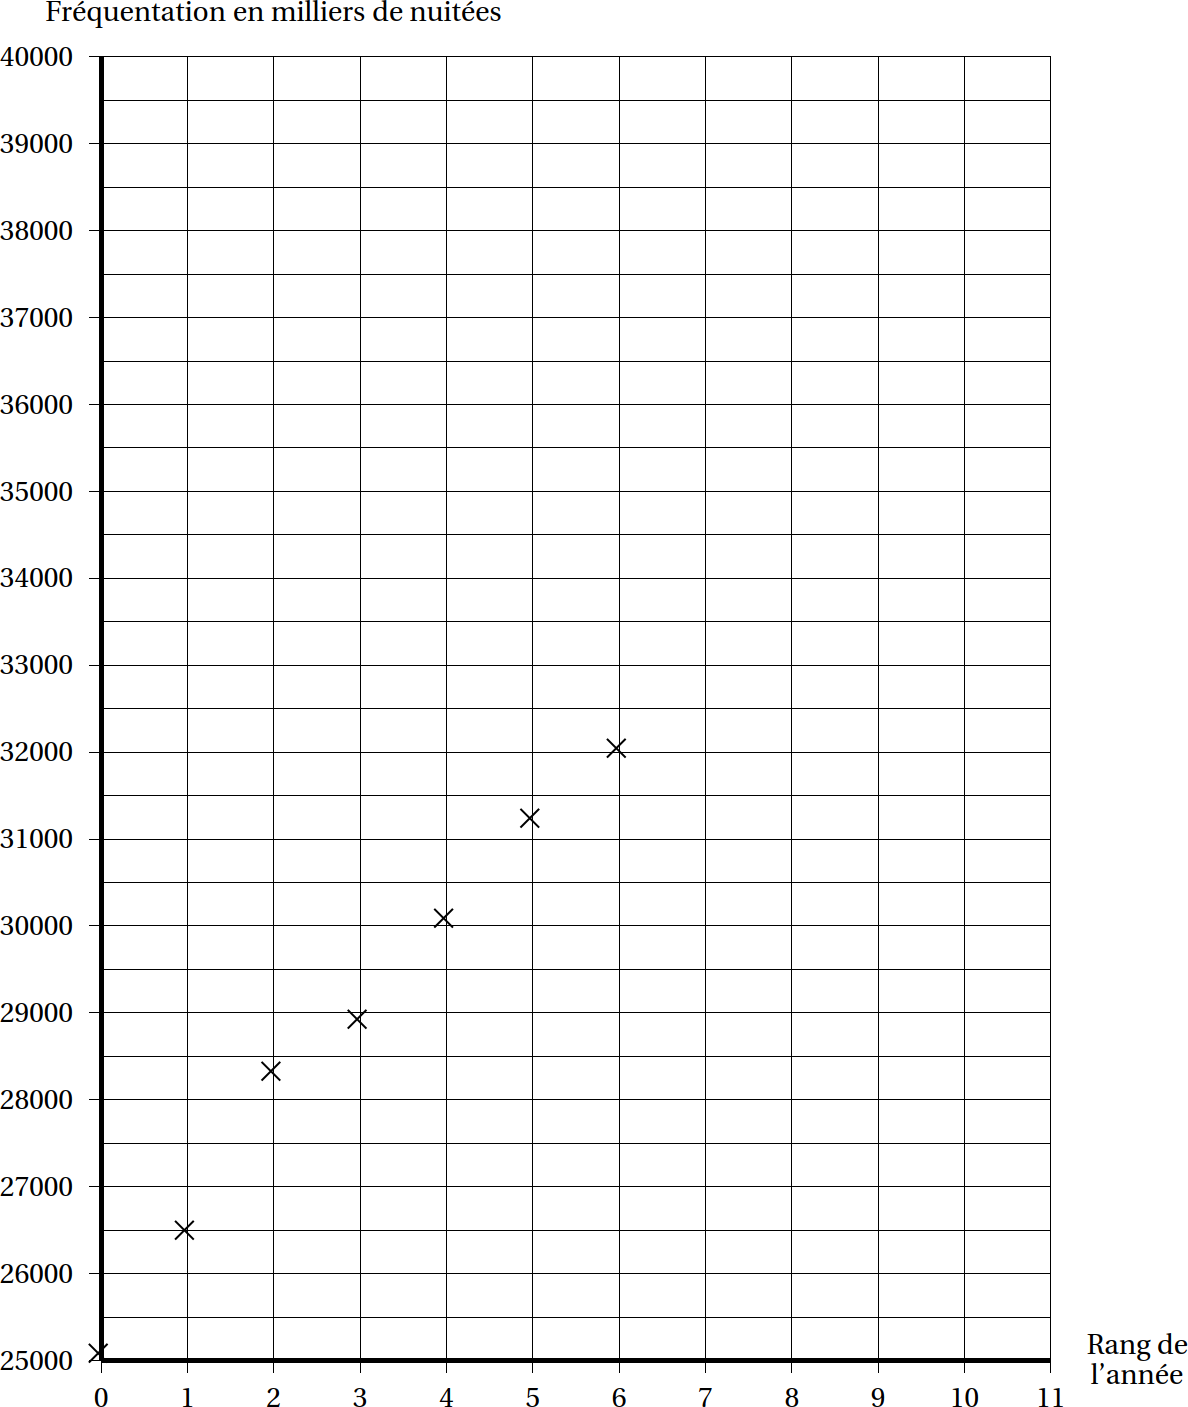
\includegraphics[width=18.5cm]{img/annexe}\end{center}
\end{document}
